\documentclass[conference]{IEEEtran}
\IEEEoverridecommandlockouts
\usepackage{cite}
\usepackage{amsmath,amssymb,amsfonts}
\usepackage{algorithmic}
\usepackage{graphicx}
\usepackage{textcomp}
\usepackage{xcolor}
\usepackage[hidelinks]{hyperref}
\usepackage{orcidlink}
\def\BibTeX{{\rm B\kern-.05em{\sc i\kern-.025em b}\kern-.08em
    T\kern-.1667em\lower.7ex\hbox{E}\kern-.125emX}}

\begin{document}

\title{\[DRAFT\] \\ ROME Connected: \\ A Network-enabled Robotics Platform}

\author{
  \IEEEauthorblockN{1\textsuperscript{st} Osvaldo Santana Neto}
  \IEEEauthorblockA{\textit{Engineering Lab UniCuritiba} \\
  \textit{Centro Universitário Curitiba (UniCuritiba)}\\
  Curitiba, Brazil \\
  \href{https://orcid.org/0009-0007-0417-2175}{ORCID: 0009-0007-0417-2175}
}
\and
  \IEEEauthorblockN{2\textsuperscript{nd} Carlos Eduardo Magrin}
  \IEEEauthorblockA{\textit{Engineering Lab UniCuritiba} \\
  \textit{Centro Universitário Curitiba (UniCuritiba)}\\
  Curitiba, Brazil \\
  \href{https://orcid.org/0009-0004-7734-5573}{ORCID: 0009-0004-7734-5573}}
}

\maketitle

\begin{abstract}
This paper presents "ROME Connected," an evolution of the ROME (\textit{Robótica Móvel nas Escolas} -- Mobile Robotics in Schools) educational robotics project. Although the original platform introduced robotics to high school students using the \texttt{ATmega328P} microcontroller with the Arduino Platform, the post-pandemic semiconductor crisis required a hardware review. This work details the transition to an \texttt{ESP32}-based architecture, driven by cost-effectiveness and the requirement for IoT (Internet of Things) connectivity. The platform provides a low-cost, open-source, scalable solution for teaching robotics, web programming, MQTT, and networking, targeting accessibility in STEM education.
\end{abstract}

\begin{IEEEkeywords}
Educational Robotics, \texttt{ESP32}, IoT, Low-cost Platforms, Open Source Hardware.
\end{IEEEkeywords}

\section{Introduction}

Educational robotics is a tool to develop skills in Science, Technology, Engineering, and Mathematics (STEM), as well as critical thinking and problem-solving \cite{rome_cotb}. The original ROME project (\textit{Robótica Móvel nas Escolas} -- Mobile Robotics in Schools) aimed to democratize access to these technologies in Brazilian public schools through a low-cost, open-source platform \cite{rome_original}.

However, the global landscape of electronics manufacturing changed following the COVID-19 pandemic. Supply chain disruptions exposed vulnerabilities in global production, leading to a scarcity of semiconductor components and significant price volatility \cite{hbr_supply_chain, semi_crisis_academic}. Legacy 8-bit microcontrollers, such as \texttt{ATmega328P}, were particularly affected by these market fluctuations mainly in developing countries like Brazil that rely on importing these components.

At the same time, educational requirements expanded beyond basic electronics to include connectivity, the Internet of Things (IoT), and network programming. To address these economic and pedagogical factors, this paper presents "ROME Connected." This project builds upon the previous version and replaces the 8-bit architecture with the 32-bit \texttt{ESP32} microcontroller (Fig. \ref{fig:esp32}) with support for multi-protocol wireless communication.

\begin{figure}
    \centering
    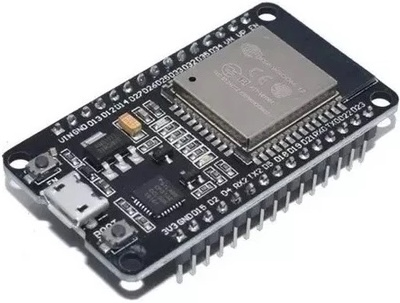
\includegraphics[width=0.75\linewidth]{esp32-wroom-devkit-v1.jpeg}
    \caption{\texttt{ESP32-WROOM} DevKit V1 (\texttt{ESP32-D0WDQ6})}
    \label{fig:esp32}
\end{figure}

The contributions of this work are as follows:

\begin{itemize}
    \item A comparative analysis of component costs and availability.
    \item The hardware design of an \texttt{ESP32}-based robotics mainboard that integrates 3.3V logic with 5V peripherals.
    \item The implementation of a motor driver solution (\texttt{MX1508}) that addresses documentation limitations.
    \item The inclusion of 3D printing alternatives for the mechanical structure.
\end{itemize}

\section{Background and Motivation}

\subsection{The Original ROME Project}

The original ROME platform consists of a differential drive mobile robot. It features a chassis made of laser-cut MDF or plexiglass, selected for low cost and assembly without screws \cite{rome_cotb}. The electronics rely on the \texttt{ATmega328P}, utilizing an \texttt{L293D} or \texttt{TB6612} H-bridge for motor control and an \texttt{HC-SR04} sensor for obstacle avoidance. It served the purpose of introducing programming, electronics, and construction.

\subsection{The Semiconductor Crisis and Cost Analysis}

The logistical challenges induced by the pandemic significantly impacted component costs worldwide, with acute repercussions on the Brazilian market. Research indicates that supply chain disruptions disproportionately affected mature technologies, as manufacturers prioritized high-margin products \cite{semi_crisis_academic}. Locally, the severe scarcity of \texttt{ATmega328P} drove the cost of standard Arduino development boards to parity with \texttt{ESP32} solutions.

This market distortion rendered the legacy architecture economically disadvantageous, given that the \texttt{ESP32} offers vastly superior specifications—including dual-core processing, expanded memory, and native communication peripherals—for an equivalent investment. To validate this strategic shift, a market survey conducted for the project identified \texttt{ESP32-WROOM-32 DevKit V1} as the optimal alternative. The data highlighted a stable supply chain for this module, with an average unit price of approximately R\$ 39.90. This finding confirmed that migrating to a 32-bit architecture was the most effective pathway to uphold the project's low-cost philosophy without compromising availability.

\subsection{Demand for Connectivity}

Emerging educational demands included network interaction and communication with robots, requirements that were practically impossible with the legacy platform limited to offline operation or basic serial interfaces. With the platform migration and the availability of connectivity resources, it becomes possible to address the following subjects:

\begin{itemize}
    \item \textbf{IoT protocols:} Using MQTT to communicate with cloud dashboards.
    \item \textbf{Web Servers:} Hosting control interfaces directly on the robot.
    \item \textbf{Wireless Networking:} Use of the \texttt{ESP-NOW} and 802.11 standards.
\end{itemize}

\section{System Architecture}

The ROME Connected platform consists of a mechanical structure, a custom Printed Circuit Board (PCB), and selected modules.

\subsection{Component Selection}

The selection process prioritized availability in the national market and ease of manual assembly. Table \ref{tab:components} summarizes the components.

\begin{table}[htbp]
\caption{Key Components Comparison}
\begin{center}
\begin{tabular}{|c|c|c|}
\hline
\textbf{Subsystem} & \textbf{Original ROME} & \textbf{ROME Connected} \\
\hline
Microcontroller & \texttt{ATmega328P} (8-bit) & \texttt{ESP32-WROOM} (32-bit) \\
\hline
Voltage Logic & 5V & 3.3V (requires shifting) \\
\hline
Motor Driver & \texttt{L293D} / \texttt{TB6612} & \texttt{MX1508} \\
\hline
Connectivity & Serial & Wi-Fi \& Bluetooth \\
\hline
Structure & Laser-cut MDF & Laser-cut MDF or 3D Print \\
\hline
\end{tabular}
\label{tab:components}
\end{center}
\end{table}

The \texttt{MX1508} was selected as the H-Bridge driver due to its compact size and cost (R\$ 19.99) compared to the \texttt{L293D}/\texttt{L298} (approximately R\$ 28.00).

\subsection{Electronic Design and Challenges}

Migration to \texttt{ESP32} introduced challenges related to voltage mismatch and component documentation.

\subsubsection{Logic Level Shifting}

The \texttt{ESP32} operates at 3.3V logic, whereas the educational sensor ecosystem (e.g., \texttt{HC-SR04}) and drivers often operate at 5V. Direct connection risks damaging \texttt{ESP32} GPIOs.

To address this, we integrated a logic level shifting stage. We utilized \texttt{BSS138}-based level shifter modules (Fig. \ref{fig:shiftlevel}). These are available, cost-effective (R\$ 12.99 for 4 channels), and enable bidirectional communication between the 3.3V microcontroller and 5V peripherals.

\begin{figure}
    \centering
    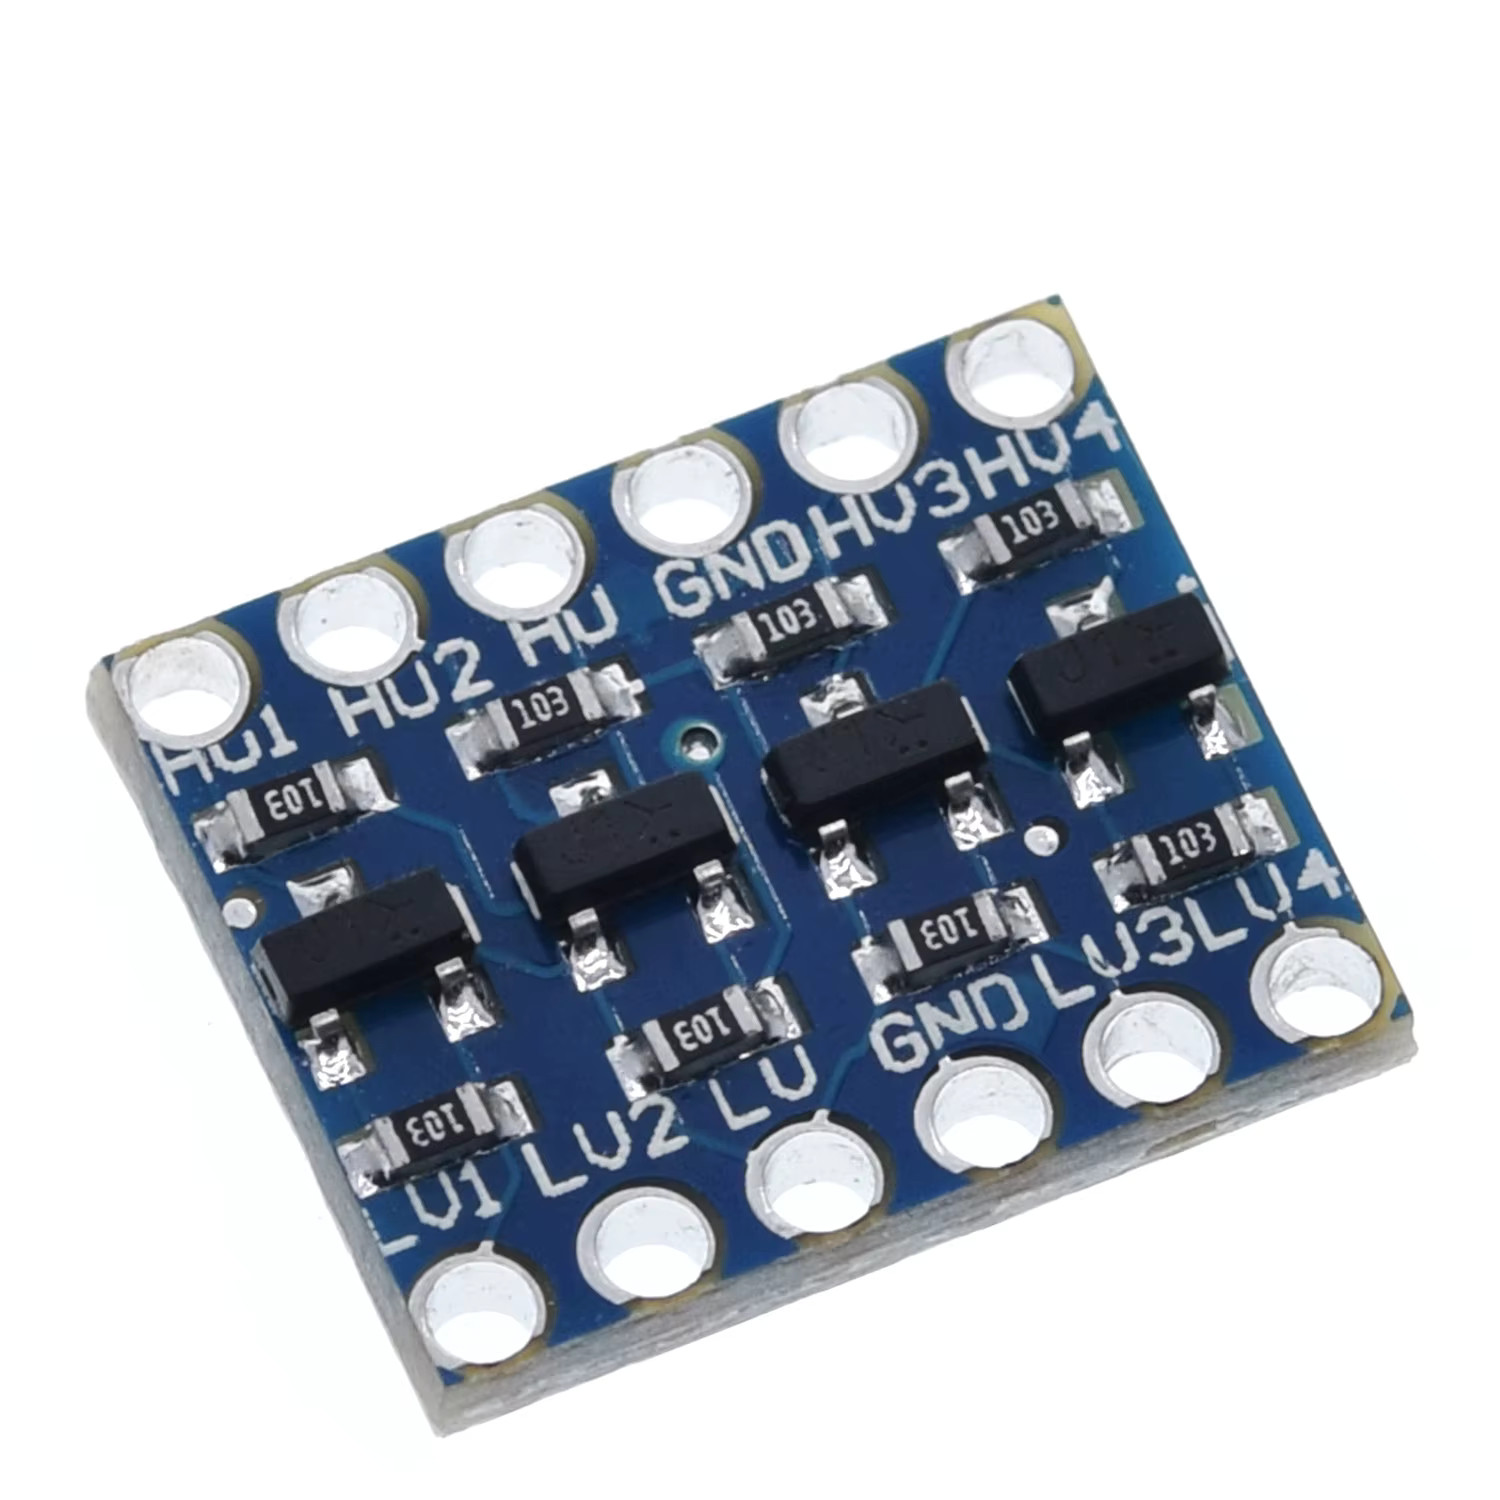
\includegraphics[width=0.5\linewidth]{shift-level.jpeg}
    \caption{Shift Level Module with 4x \texttt{BSS138}}
    \label{fig:shiftlevel}
\end{figure}

\subsubsection{Motor Driver Integration (\texttt{MX1508})}

The \texttt{MX1508} module was selected for its efficiency and cost-effectiveness. However, a significant limitation was the scarcity of comprehensive documentation; datasheets were primarily available in Chinese, and standard Arduino libraries presented incompatibilities with PWM support.

We analyze the control signals to develop the integration. The \texttt{ESP32} utilizes Pulse Width Modulation (PWM) on the driver's input pins to control the speed of two DC motors. This required the implementation of PWM channels using the \texttt{ESP32 LEDC} peripheral API .

\subsection{Mechanical Design Updates}

The MDF structure was retained for institutions with laser cutters. ROME Connected introduces a 3D-printable chassis model. This inclusion is for schools with 3D printers but without laser cutting machinery. In addition, pin headers were replaced with pin sockets to facilitate the use of standard male-to-male jumpers.

\section{Implementation Status}

\subsection{Prototyping}

The development followed three stages:

\begin{enumerate}
    \item \textbf{Breadboard Validation:} Components, including level shifters and \texttt{MX1508}, were tested on a universal circuit board to verify logic leveling and power consumption.
    \item \textbf{Schematic Design:} The circuit was defined in KiCad \cite{kicad}, incorporating the \texttt{ESP32} DevKit footprint.
    \item \textbf{PCB Design:} The PCB integrates slots for the \texttt{ESP32}, \texttt{BSS138} modules, and motor terminals.
\end{enumerate}

\subsection{Current Constraints}

A challenge involves the inconsistency among the "\texttt{ESP32} DevKit V1" boards on the market. Pinout variations require the PCB design to accommodate physical dimensions and connection differences.

\section{Conclusion and Future Work}

The ROME Connected project updates the ROME platform. Using \texttt{ESP32}, the project addresses supply chain issues affecting 8-bit microcontrollers and enables IoT education. The technical solutions for voltage leveling and driver integration maintain the affordability of the platform. Future work includes PCB validation, release of 3D printable files, and development of a curriculum module focused on web-based robot control and MQTT communication.

\bibliographystyle{IEEEtran}
\bibliography{references}

\end{document}
